\chapter{Introduction}

  \section{The chemical perception}
  Chemical perception is one of the oldest sensory systems, having evolved 500 million years ago. It mediated reproduction and feeding, two of the most fundamental animal behaviors. In fish, chemical perception passes through three distinct organs: olfaction, taste, and a common chemical sense. Unlike terrestrial species, where substances perceived by smell and taste differ by the medium of transport of the molecules, fish taste and smell through the same medium: water. The solubility of compounds in water determines the type of compounds that can be transported and perceived. The chemical perception is non-directional and persistent. The distance traveled and the perceived concentration depend on the diffusion and convection of the medium, determining the perception threshold and the compound's residence time in the environment. The chemical perception is extremely specific, being contained in the molecular structures and the complex mixture of chemicals. Therefore, we expect to observe non-directional excitation behaviors or oriented gradient upward responses to find sources, such as orienting oneself or finding a place to lay eggs during migration. This navigation is a complex task and cannot be compared to a straightforward gradient ascent, as the aquatic environment is generally turbulent and perception is fragmented.

  The zebrafish larva is the model of choice for studying chemical preference and chemically-driven navigation. In the larval stage, the animal is transparent. Therefore, it is possible to observe the entire brain with cellular resolution using light-sheet microscopy while the animal is performing a task and thus links behavior to neuronal activity. The sensory organs of chemical perception have been well characterized in the zebrafish. However, there are few behavioral studies on chemical perception and chemically-oriented navigation. The model is widely used in addiction-related studies due to the ease of genetic manipulations and its low cost. An animal model's characterization to study chemically oriented navigation, linking behavior to neuronal activity, would be a powerful addition to our understanding of how fish perceive and travel back to food sources, spawning, and migration sites.

    \subsection{Olfaction}
    The olfactory organ of the fish Figure~\ref{olfactory_schematic} consists of two structures located in the animal's snout. Each structure consists of a cavity called the olfactory chamber connected to the outside by an entrance and an exit nostril. The inside of the olfactory chamber is lined with the olfactory rosette consisting of two rows of olfactory lamellae. The olfactory epithelium, where the olfactory receptors are located, is placed on these lamellae. The olfactory organ's exact organization and position can vary depending on the fish species, for example, with the addition of a ventilation cavity as an extension of the olfactory cavity.

    \begin{figure}[h]
      \centering
      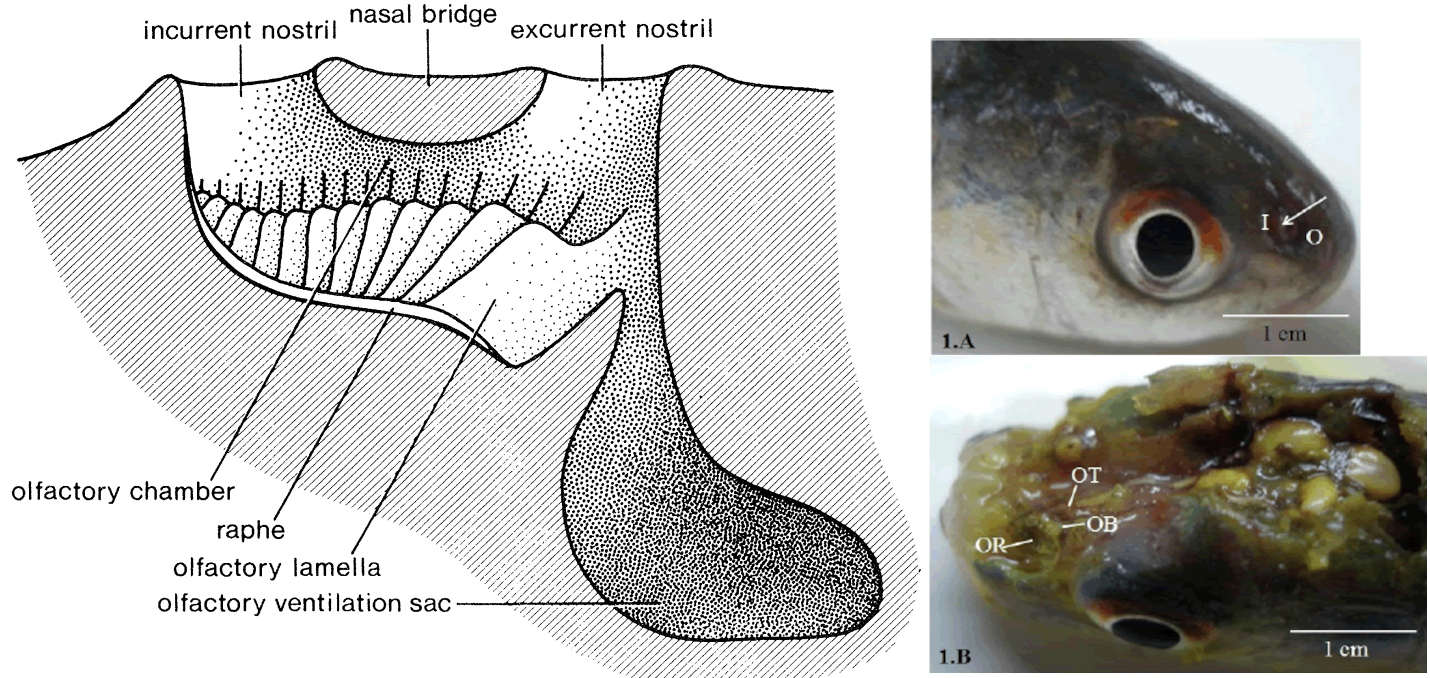
\includegraphics[width=10cm]{part_2/assets/olfactory_schematic.png}
      \caption{Olfactory system, reproduced from \cite{hara2012fish}.}
      \label{olfactory_schematic}
    \end{figure}


    The olfactory epithelium has a $100\mu m$ thick stratified columnar structure. It can be separated into a sensory and a non-sensory epithelium. The sensory epithelium consists of three types of cells: receptor, supporting, and basal cells; the non-sensory epithelium of goblet cells and non-sensory ciliated cells. There are five receptor cells implicated in the olfactory perception: ciliated cells, microvillous cells, crypt cells \cite{ichikawa1977fine,hansen2005diversity}, kappe cells \cite{ahuja2014kappe}, and pear-shaped cells \cite{wakisaka2017adenosine}. They express olfactory receptors of the OR, V1R, V2R, and TAAR families. Receptor cells have various sizes, shapes, and distribution inside the epithelium see Figure~\ref{olfactory_schematic_full}.

    \begin{figure}[h]
      \centering
      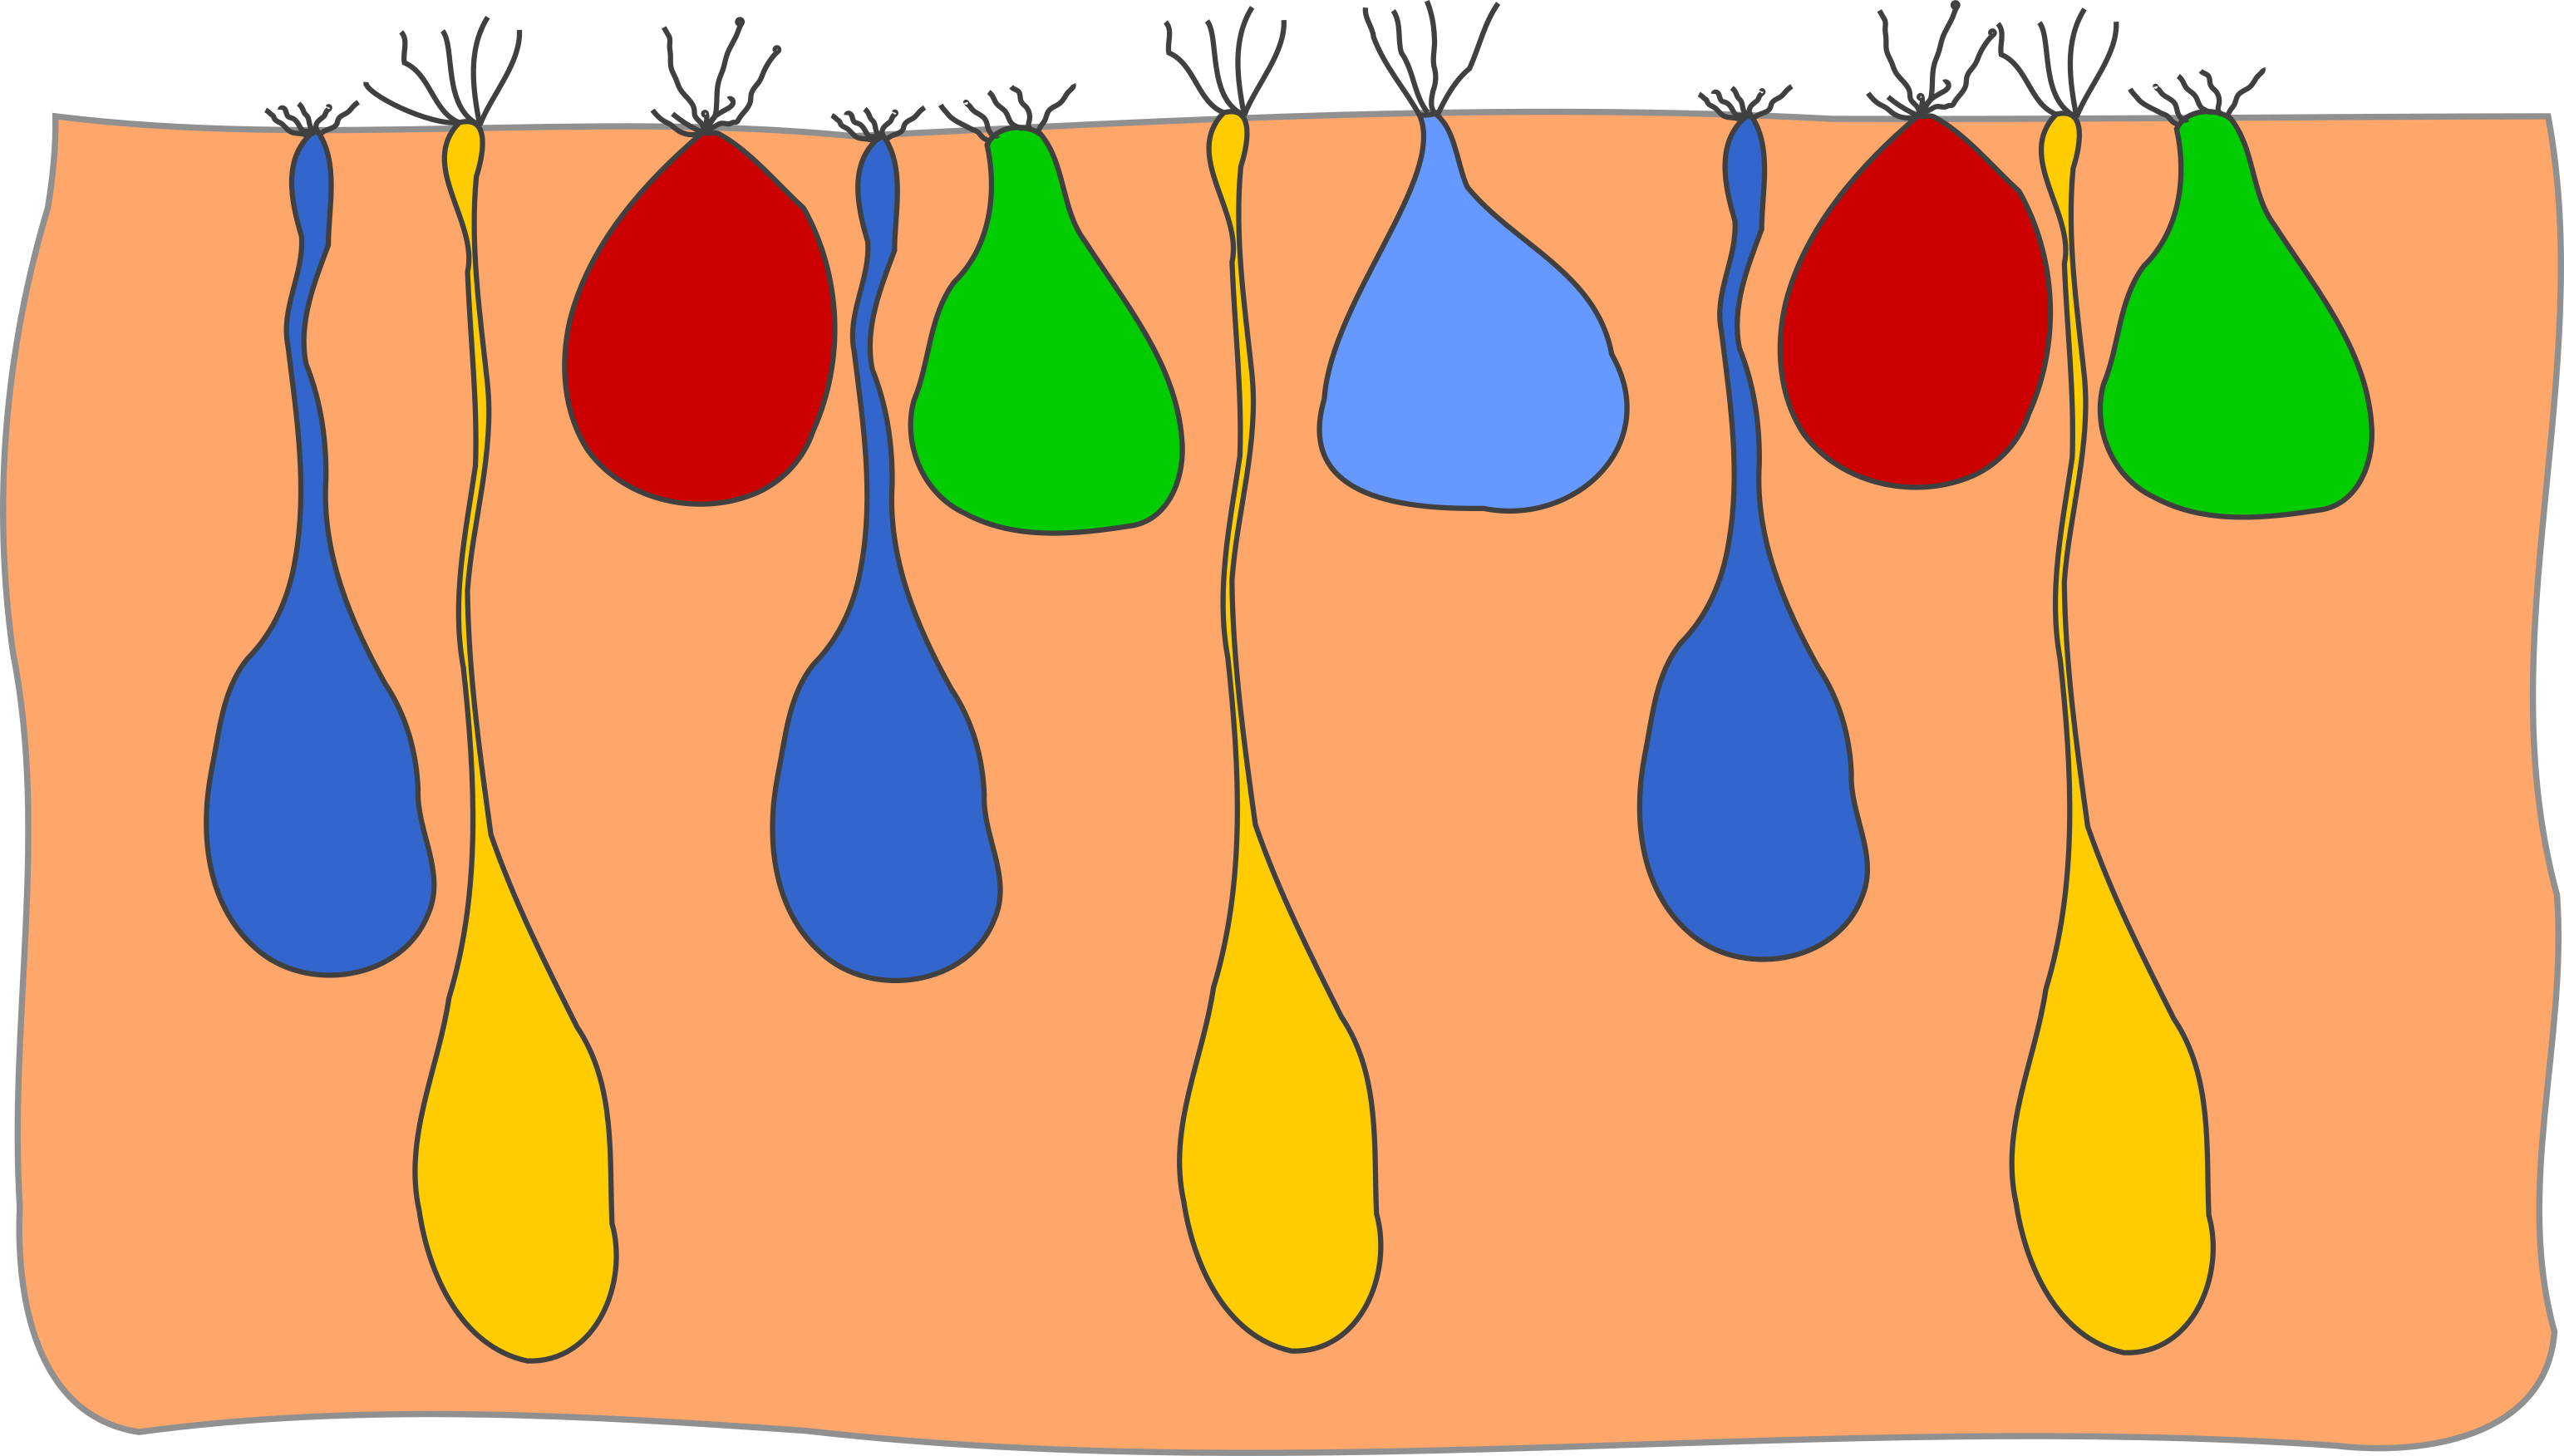
\includegraphics[width=10cm]{part_2/assets/olfactory_schematic_full.png}
      \caption{{\bf Schematic representation of the olfactory epithelium.} Ciliated neuron in yellow with round somata, slender dendrite, and cilia. Microvillous neuron in dark blue with microvilli at the surface. Crypt neuron in red with ovoid shape, microvilli, and cilia. Kappe neuron in green with microvilli. Pear-shaped neuron in light blue with cilia.}
      \label{olfactory_schematic_full}
    \end{figure}

Receptor cells project directly into the olfactory bulb located in the brain, in turn sending signals to the telencephalon and diencephalon \cite{miyasaka2009olfactory}. The olfactory bulb in the teleost is a structure of four concentric layers: olfactory nerve layer (ONL), glomerular layer (GL), mitral cell layer (MCL), and internal cell layer (ICL). The olfactory information is transmitted by the receptor cells to the olfactory bulb \cite{nikonov2001electrophysiological} then in the forebrain \cite{nikonov2005beyond} as a topographical odor map. The olfactory bulb's neuronal connections have been particularly studied in the zebrafish \cite{hansen1998peripheral,kermen2013neural}, the olfactory bulb comprised approximately 20 000 neurons \cite{friedrich2009processing} and 140 glomeruli\cite{braubach2012distribution}. Each receptor cell expresses only one type of olfactory receptor \cite{serizawa2004one,barth1997noncoordinate,weth1996nested,sato2007hierarchical} except in a subpopulation of olfactory sensory neurons \cite{sato2007hierarchical}. Cells expressing the same receptor are projecting into the same olfactory bulb glomeruli \cite{sato2005mutually}. Glomeruli responding to similar odorants are grouped into domains within the olfactory bulb, forming chemotopic maps. Odorants can activate glomeruli outside their domain, leading to a fragmented map inside the olfactory bulb \cite{friedrich1998chemotopic}. Moreover, the odor encoding is hierarchized with first-order features encoded by large domains and second-order features by local activity patterns within the domain \cite{fuss2001odorant,korsching2001odor}.

    The olfactory bulb projects into two higher brain structures, the telencephalon (Dp and Vv) and the diencephalon (habenula, posterior tubercle, and hypothalamus). Odor response in these areas is currently poorly understood.

    In the zebrafish \cite{hansen1993development,miyasaka2013functional}, the olfactory organ develops from the olfactory placodes at the 6-10 somites stage (about 15 hours post-fertilization) of the embryonic development. The olfactory cavity begins to appear at the 28-30 somites stage (31 hours post-fertilization). Approximately 50 hours post-fertilization, the olfactory epithelium and the receptor cells appear. When the embryo emerges from the egg, 4 days post-fertilization, the olfactory organ continues its morphological development, but the cytological organization changes little. At 40 days post-fertilization, the bridge between the entrance nostril and the exit nostril is completely formed, separating the currents going out and coming in from the olfactory cavity. The addition of lamellae to the olfactory rosette continues throughout the life of the zebrafish.

    \subsection{Gustation}
    The gustatory organ of fish consists of the taste buds, which directly contact chemical substances. Taste bud histology has been studied for different fish \cite{kapoor1976gustatory,fishelson2004taste,reutter2000heterogeneity,reutter1991ultrastructure,reutter2012taste}. They usually have an elongated and ovoid shape. They sit on a small dermal papilla and extend throughout the epidermis' thickness protruding from the surface. The taste bud is constituted of a sensory (dark cells with microvilli and light cells with one large microvillus) and a non-sensory (Merkel‐like basal cells) epithelium. The apical ending of the sensory cells that protrude from the epithelium is called the receptor field and covers with a mucous cap. The number of sensory cells in a taste bud varies considerably depending on the fish species.

    Taste buds are distributed all over the fish's body, especially in the mouth, on the lips, and the skin. Their distribution and concentration vary according to the species. Three different cranial nerves innervate them: facial (VII), glossopharyngeal (IX), and vagal (X). The facial nerve transmits information from the extra-oral taste buds; the glossopharyngeal nerve transmits information from inside the oral cavity; the vagal nerve transmits information from inside the oropharyngeal cavity. The taste system is anatomically divided into two distinct parts: nerves IX and X projecting into the brain's vagal lobe and nerve IV into the facial lobe. Connections to higher areas of the brain differ slightly from one species to another. It has been shown in Ictalurus nebulosus \cite{datema1971structures} that these two systems have distinct roles in fish feeding behavior.

    \begin{figure}[h]
      \centering
      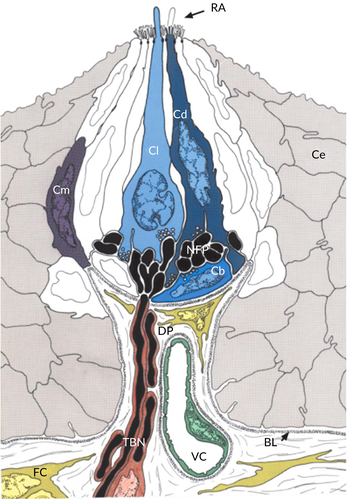
\includegraphics[width=8cm]{part_2/assets/gustatory_schematic.png}
      \caption{\textbf{Schematic drawing of a typical taste bud of teleosts from \cite{hansen2002taste}.} Dark cells (Cd), light cells (Cl) and Merkel‐like basal cells (Cb). Marginal cells (Cm). Ce epithelial cells. Dermal papilla (DP). (TBN) taste bud nerve. (BL) basal lamina. (RA) receptor area. (VC) capillary vessel.}
      \label{gustatory_schematic}
    \end{figure}

    In zebrafish \cite{ohkubo2005distribution}, the taste buds (approximately 2 200) are located on the lips, in the oropharyngeal cavity on the barbels, and on the head's ventral and dorsal side. Each taste bud contains 20 to 23 cells. Projections of the zebrafish gustatory system have been studied in detail \cite{yanez2017gustatory} and form a complex network that can be summarized graphically see Figure~\ref{gustatory_connection_schematic}.

    \begin{figure}[h]
      \centering
      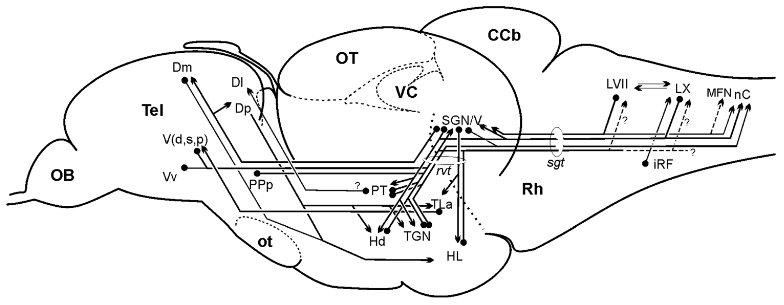
\includegraphics[width=10cm]{part_2/assets/gustatory_connection_schematic.png}
      \caption{\textbf{Gustatory system of the zebrafish}. Neuronal connections of the fish taste system reproduced from \cite{yanez2017gustatory}.}
      \label{gustatory_connection_schematic}
    \end{figure}

    The development of the gustatory organ has been studied in the zebrafish \cite{hansen2002taste}. The first taste buds appear at 3 or 4 days post-fertilization and are located on the lips and the gill arches. The taste buds in the mouth and oropharyngeal cavity appear 4 to 5 days post-fertilization. The taste buds on the head do not appear until 12 days post-fertilization, and it is not until the juvenile stage (30 to 40 days post-fertilization) that the barbels appear. Note that the appearance of the taste buds coincides with the appearance of feeding in the larvae.

    \subsection{Commom  chemical sense}
    Fish also have a third chemical sense called the common chemical sense. It consists of bipolar neurons called solitary chemosensory cells (SCCs) embedded in the epidermis. Their distribution and number vary greatly depending on the species. Therefore their study is difficult, and their function and neuronal connections are poorly understood.

    In the zebrafish \cite{kotrschal1997ontogeny}, SCCs have been described as a set of 2-7 villi of 0.5 to 1 $\mu m$ length emerging from the cell body at embryo and larval stage.  In adults, SCCs possess a single villus of $3\mu m$ length.

    The first SCCs appear at 3 days post-fertilization. Their density increases until 25 days, where their number stabilizes at $1.10^6$ per $mm^2$ with 2 to 5 times more SCCs on the zebrafish's head than on its body.

    \subsection{Behavior}
    The olfaction and gustation have been shown to mediate several fish behaviors. It is not easy to distinguish the contribution of each sense in the observed behavior. Moreover, this contribution seems to be dependent on fish species.

    A well known and impressive behavior encountered in many fish species is the homing migration. A typical example is salmons that perform three migratory phases throughout their life. One of them, the upstream migration from the ocean to their home stream, has been shown to rely on an olfaction imprinting \cite{stabell1992olfactory,hasler1983olfactory}. Little is known about the imprinting mechanism, but experiments suggest that it relies on a mixture of odors perceived during the juvenile stage in the fish's home stream.

    Feeding is one of the most important behaviors. It relies on several senses for food detection, and selection \cite{pavlov1990sensory}. A stereotyped behavioral sequence was shown to exist \cite{atema1980chemical} consisting in a step of arousal mainly mediated by olfaction \cite{bateson1890sense}, then a step of localization of the food mediated by chemical and visual cues. The last step of ingestion is triggered primarily by the gustation \cite{atema1980chemical}. The impact of each sensory modality varies significantly with the species. For example, the yellow bullhead has the entire feeding sequence mediated by taste, whereas ictalurid catfish prey detection was abolished when olfaction was blocked. The chemical substances that attract fish depend on the species \cite{atema1980chemical}, and response to a mixture is higher than isolated compounds in general.

    Olfaction \cite{tavolga1956visual} as well as the gustatory system \cite{de1983influence} has been shown to play an essential role in reproduction. Non-anosmic males exposed to water taken from a tank with a gravid female developed courtship behaviors, except for some species like the three-spined stickleback where the gustation can replace the olfaction. Complete courtship repertoire necessitated the presence of other sensory cues.

    Fright reaction occurred when a fish perceived an alarm substance secreted by a conspecific. This reaction differs between species and involves seeking cover, rapid swimming, or freezing. It is accepted to be mediated by olfaction \cite{frisch1942schreckstoff,speedie2008alarm,doving2009alarm}, but other sensory cues are not ruled out.


  \section{Behavioral studies}
  The zebrafish has been used to connect the behavioral and neuronal response to diverse stimuli: visual stimuli \cite{}, temperature \cite{}, and balance reflexes \cite{}. Most of the works to date focus on developing the model for pharmacological safety screening \cite{cassar2019use}, drugs addiction \cite{klee2012zebrafish}, and ecology \cite{dai2014zebrafish}, enabling a low cost and genetically manipulable model. Behavioral studies of the chemical perception of zebrafish, adults, or at the larval stage have been done through various experimental apparatuses that we will present in the following sections.

    \subsection{Conditioned place preference}
    The conditional place preference (CPP) experiment is a type of Pavlovian conditioning. Pavlovian conditioning consists of associating a conditioned stimulus (generally neutral) with an unconditioned stimulus. After learning, the animal exhibits a conditioned response to the conditioned stimulus when presented alone. The most classic example is associating a bell's sound (conditioned stimulus) to the release of a food smell (unconditioned stimulus). After learning, the animal can respond to the bell's sound alone.

    This approach was applied to test the response to various chemical stimuli in adult zebrafish \cite{mathur2011conditioned}. The experiment follows a classical 3-step design. The first step is to evaluate the fish's base-line preference. The animal is placed in an aquarium with two or three distinct areas differentiate by walls' pattern and color, see Figure~\ref{cpp_schematic}. The fish is tested to find out which side it naturally prefers. In this experiment, the distinctive walls' pattern and color play the role of the conditioned stimulus. The second step is the conditioning phase. The fish is restrained to its least preferred area, and the substance to be tested injected into the water (unconditioned stimuli). The last step consists of repeating the first step to assess the change in preference of the animal.

    Several chemical substances have been tested using this method \cite{blaser2014experiments,collier2013utility,tzschentke2007review}. Notably, a strong and robust cocaine-induced CPP response in WT zebrafish was shown \cite{darland2001behavioral}, with $85\%$ of the fish changing preference to a cocaine concentration of $10mg.L^{-1}$ and lower and higher concentrations resulting in a lower response. A positive response of adult zebrafish to a single ethanol exposure was shown \cite{mathur2011preference} in a similar experimental setup. It should be noted that this is also the first study to use an automated tracking system to calculate animal preference. Zebrafish showed a positive response for D-amphetamine \cite{ninkovic2006genetic, ninkovic2006zebrafish}, salvinorin A \cite{braida2007hallucinatory}, cocaine \cite{braida2007hallucinatory}, spiradoline \cite{braida2007hallucinatory}, nicotine \cite{kedikian2013behavioral} and ethanol \cite{kedikian2013behavioral}.

    We see that CPP has been used extensively to study the response to chemical stimuli in zebrafish. There is a strong emphasis on products that cause addictive pathologies in humans. Nevertheless, this protocol has several flaws, the first being that it involves several systems of perception as well as memory. During the conditioning phase, the learning is based on the visual perception of the environment (pattern on the aquarium walls), the chemical perception of the tested compound, the association of the two stimuli coming from different sensory organs, and the memorization of these perceptions. Secondly, the time window to perform the experiment (minimum two days) is a hindrance to use the CPP to study the effect of many chemicals in a high-throughput manner.

    \begin{figure}[h]
      \centering
      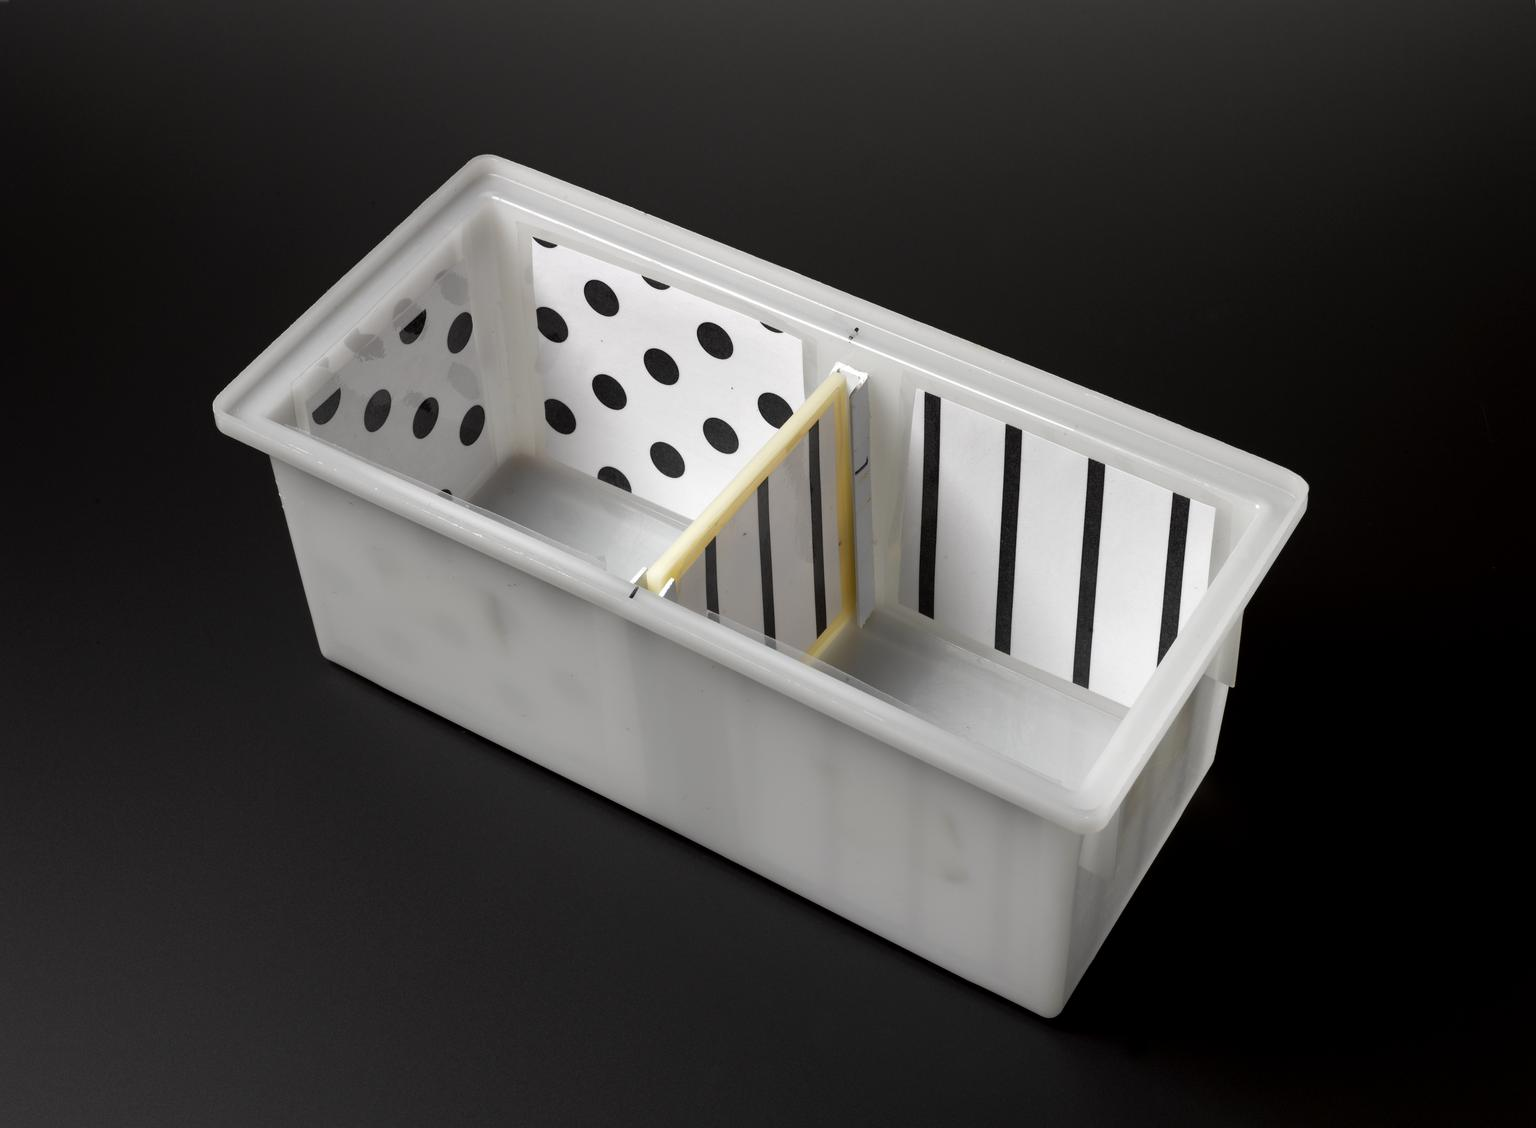
\includegraphics[width=0.8\textwidth]{part_2/assets/cpp.jpg}
      \caption{\textbf{Conditioned place preference apparatus}.  CPP setup for zebrafish reproduced from Brennan Caroline, Queen Mary University of London. The middle wall is removed for the first and third step of the CPP.}
      \label{cpp_schematic}
    \end{figure}

    \subsection{Well-plate}
    A widely used experimental apparatus to assess chemical compounds' effect on zebrafish larvae and embryos is the well-plate device \cite{rennekamp201515}. One or more larvae is placed in each well in a bath of a chemical. Larvae are then recorded swimming in the chemical compound, and the kinematic parameters of the animal are extracted. In the case of embryos, development is monitored after exposure. The advantage of this technique is that it requires little equipment. It quickly produces a large amount of data with well-plate up to 48 wells per plate. Software already exist to extract automatically relevant behavior parameters from video recordings.

    With this device, many chemical compounds have been tested \cite{sallinen2009mptp,rihel2010zebrafish,kokel2010rapid}, as well as seizure liability \cite{winter2008validation}, and several behaviors \cite{farrell2011evaluation, shen2020rapid,schnorr2012measuring,pelkowski2011novel}.

    The well-plate device allows an easy and automatic high-throughput screening of chemicals. Turnkey commercial solutions like the Zebrabox from ViewPoint exist, and custom setups are relatively easy to build. However, this system suffers limitations like the fact that one can not assess the fish preference. Precisely controlled exposure, or repeated exposure through cycles of exposition/flushing, are not available. Therefore this system is not adapted to investigate fish's chemical preference and chemical-driven navigation.

    \begin{figure}[h]
      \centering
      \includegraphics[width=0.4\textwidth]{part_2/assets/well.png}
      \caption{\textbf{A Zebrabox from Viewpoint}.  Zebrabox, the most used solution for well-plates experiments.}
      \label{gustatory_connection_schematic}
    \end{figure}

    \subsection{Diffusion}
    Some authors have tried to quantify chemically induced behavior by introducing a chemical compound directly into the tank and looking at the percentage of time spent close to the source. Notably, an attraction concentration-dependent to adenosine for adult zebrafish\cite{wakisaka2017adenosine} and to GCDA and nicotine for zebrafish larval \cite{krishnan2014right} was shown. A strong aversion to cadaverine, an odor associated with decomposing bodies, was shown using a tank with a single compartment or a tank with two compartments and an intermediate zone where the fish can changes compartment \cite{hussain2013high}, see Figure~\ref{diffusion_setup}.

    Very easy to implement, these types of experimental devices lack control in the concentration perceived by the animal. Diffusion and convection are neglected in the experiment, and the concentration is poorly known and not reproducible. The effect of diffusion and convection was mitigated \cite{hussain2013high} by adding a wall separating the two zones Figure~\ref{diffusion_setup}.F, always leaving uncertainty in the intermediate zone. Moreover, these setups exclude the realization of long experiments due to the homogenization of the product.

    \begin{figure}[h]
      \centering
      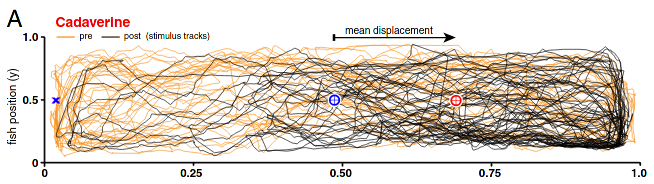
\includegraphics[width=1\textwidth]{part_2/assets/diffusion.png}
      \caption{\textbf{Diffusion setups from \cite{hussain2013high}}. \textbf{A.} One channel diffusion setup, blue cross: chemical introduction point. \textbf{F.} Two channels setup.}
      \label{diffusion_setup}
    \end{figure}

    \subsection{Flow}
    An exciting setup to study chemical preference in fish is the underflow device. The first mention of this type of device date back to 2013 \cite{readman2013fish}. In this setup, the tank is separated into two distinct compartments using a laminar flow, see Figure~\ref{flow_0_setup}. The animal can then choose between the two compartments during the experiment without any constraint, and the experimenter can put a chemical to test on one side. The interface between the two compartments self-heal with a characteristic time depending on the flow velocity. The time spent on each side, the number of interface crosses, and the animal's kinematic parameter are extracted from video recordings to assess the fish's preference.

    Several psychoactive substances have been tested on adult zebrafish \cite{abreu2016acute, abreu2016behavioral} and showed attraction by diazepam, fluoxetine, risperidone, and buspirone; neutral response to ethanol and clonazepam; an aversion to acid pH, two food odor extracts, and conditioned water took from a tank with chemically and physically stressed fish.

    This setup has several advantages. The concentration of the product is perfectly known because the diffusion and convection are prevented by the flow. The preference of the fish can be directly assessed because the fish can choose freely to go inside or outside the product. Long experiments can be performed with this setup, and product delivery precisely controlled in time. However, some disadvantages remain, like the absence of a standardized or turnkey setup and the volume of water and chemicals required that can be high.

    \begin{figure}[h]
      \centering
      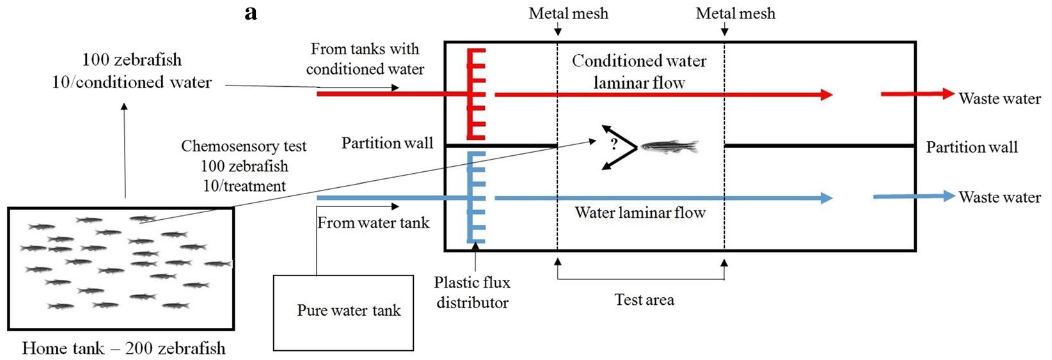
\includegraphics[width=1\textwidth]{part_2/assets/flow_0.png}
      \caption{\textbf{Flow setups from \cite{abreu2016behavioral}.}}
      \label{flow_0_setup}
    \end{figure}

    Another type of flow device that allows the product's concentration inside the tank to be quickly changed was used on adult zebrafish \cite{kermen2020stimulus}. Like in the multi-well experiment, chemically induced behavior changes were monitored by the animal's kinematic parameters.

    Several food odors were shown to produce a significant increase in speed and number of bursts; social odors from conspecific produced a similar response; alert odors result in a dive to the bottom of the tank and an increase in frozen time; decomposition odors result in more turns. The critical points noted with this device is the inter-and intra-experimental variability. The authors showed that less than a third of the odors used in the study produce reproducible results between trials of the same individual. Some odors such as cadaverine, blood, skin, and food odors resulted in inconsistent responses for the same individual. Most odors produce poorly reproducible results for different fish.

    \begin{figure}[h]
      \centering
      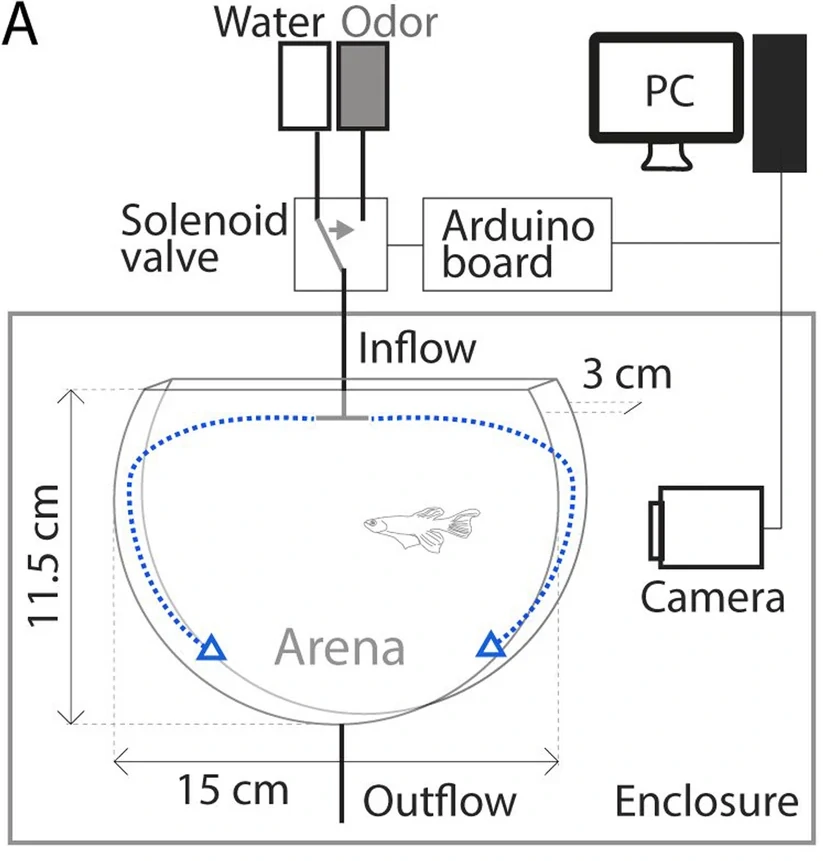
\includegraphics[width=0.5\textwidth]{part_2/assets/flow_1.png}
      \caption{\textbf{Flow setups from \cite{kermen2020stimulus}.}}
      \label{flow_1_setup}
    \end{figure}

    This setup novelty is to allow adult animals to evolve realistically in a 3D environment and to have a better knowledge of the concentration perceived by the animal than in a diffusion setup. Therefore, direct preference assessment is not accessible, and comparisons with existing quasi-2D setups like the well-plate are difficult.

    From this overview of the scientific literature, we see that the study of chemical perception and behavioral response to chemical stimuli is not standardized. No experimental setup is set as a standard, and direct comparisons between studies carried out in various independent laboratories are not easily possible. In this context, we have developed Dual, an open-source, low cost, do it yourself, and scalable experimental setup. Using the underflow principle, Dual allows studying chemical preferences in larvae and juvenile zebrafish in a standardized, high-throughput, and comparable way.

\chapter{Experimental setups}

  \section{Dual}
  The comparison of behavioral studies is an open problem in neuroscience. The design and implementation of experimental setups that are high-throughput, avoiding bias, and scalable are essential to behavior characterization. The absence of a standardized setup to assess chemical stimuli preference does not allow easy comparison through various studies already published. We present Dual, a high-throughput experimental setup that is easy to set up and implement.

  \subsection{Overview}
  Dual is an underflow system builds on the same principle that \cite{readman2013fish}. It consists of creating two virtual compartments in a tank through a laminar flow. As we have seen previously, this system allows a rigorous knowledge of the compound's concentration to which the animal is subjected. Diffusion and convection due to the water movements caused by the fish are avoided. The interface between the two compartments is well defined and self-heal, when disturbed, with a characteristic time depending on the flow.

  To create the laminar flow, Dual uses a system of four syringes, coupled by two, in phases opposition, when two syringes push, two syringes pull, see Figure~\ref{}. The syringes are connected to a millifluidic chip, where the fish is placed, and generate a laminar flow with constant volume by having two syringes injecting at one side and two aspirating at the other side. Thanks to a microvalves system, each syringe can be filled independently. One can then build an experimental protocol by stacking several filling and injection cycles and choosing with which product to fill the syringes.

  For example, to access fish preference, one can first create a cycle with water on the two sides as habituation and control. Then add a cycle with a chemical on one side and water on the other side to study the fish preference. Another example is to fill the two sides with a chemical for a given amount of time and then clean the system with water on two sides, reproducing the type of experiment performed with the well-plate device.

  Dual is a Do It Yourself project, which allows great flexibility in the conception and fast iteration to adapt the project if necessary. All the components, blueprints, and other CAD files needed to build and assemble Dual are available in the appendixes. Dual can be built at a low-cost \ref{} without prior knowledge of mechanics or electronics. The tools necessary for the realization of the parts can be found in a FabLab.

  \subsection{Construction}
  For the construction, Dual can be separated into five inter-dependent parts. The mechanical system comprised all the structures, the motor, and moving parts. The millifluidic system is constituted of the millifluidic chip, the microvalves, the syringes, and connecting tubes.  A camera and LEDs form the imaging system. The electronic system is a custom PCB controlling the motor and the microvalves. Finally, a software that controls all the setup automatically.

  \subsubsection{Mechanical}
  Dual's central mechanical part is the motorized syringe push-pull pump that allows creating the laminar flow. It is built around the V-Slot Linear Actuator from OpenBuilds fixed on a structure builds using OpenBuilds linear rails and 3D printing fixations. A stepper motor drives the actuator, and two stop microswitches fixed on the structure limit the range of motion.

  It is crucial to isolate the animal from the exterior environment and of any light sources. A box that will contain the millifluidic chip and lighting system is constructed using MakerBeam rails and medium-density fibreboard sheets. A PMMA infrared transparent sheet is placed on the removable top panel to record the experiment while blocking visible light. The box contains, see Figure~\ref{}, two LEDs for visible and infrared light, a diffuser for homogeneous lighting, and support to fix the millifluidic chip.

  A structure to maintain the camera on top of the box and secure the Raspberry and the power alimentation is build using OpenBuilds rails. It is best to build Dual on top of an optical breadboard to facilitate fixation and enhanced stability. All these elements need to be fixed firmly and level to avoid any bias that could disturb the animal during the experiment.

  \subsubsection{Millifluidic}
  The millifluidic chip that will serve as a tank for the fish, see Figure~\ref{} is laser cutted in XXXX plastic that is transparent and presents excellent optic properties. The different parts are stick using acetic acid \cite{}. The fish is restrained in the center by nets, and profiled inputs and outputs allow a laminar flow.

  Sixty-milliliters syringes are fixed with 3D printed connectors on the actuator and connected with tubes to the microvalves circuit.

  Six three ports microvalves are connected, see Figure~\ref{}, and form a circuit that allows performing cycles of filling and injection.

  \subsubsection{Imaging}
  The setup is lightened by transmission using an infrared LED placed at the bottom of the box. Homogenous lighting is obtained by placing a diffusor (tracing papers or white plastic sheet) at the box's mid-height. Experiments are recorded with a Chameleon 3 camera mounted with a 23-25 mm EFL lens connected directly to the computer via USB3. A PMMA infrared transparent sheet is placed between the camera and the lens to block visible light and only retrieve Dual's infrared lightening.

  \subsubsection{Electronic}
  The electronic system links the analogic mechanical and millifluidic system to the software. A custom printed circuit board (PCB) has been designed for Dual \ref{}. It contains an Arduino Nano serving as a microcontroller; six half-bridge gate drivers to control the microvalves from the logic signals of the Arduino; a Big EasyDriver stepper motor controller is controlling the motor speed from a logic output of the Arduino; a potentiometer to control the intensity of the LED lighting. All the electronics and the syringe pump motor are powered by a 550W ATX computer power supply connected to the PCB.

  \subsubsection{Software}
  A software has been specifically developed to control the setup. The graphical user interface is developed using Qt, and the camera is interfaced to the software using the FLIR Systems SDK \url{} provided with the camera. The electronic system is controlled through the Arduino Nano flashed with a custom sketch \url{} and communicating to the software via USB serial. The software allows manual control of each system element, such as the microvalves, the camera, and the motor. It is possible (and advisable) to create experimental protocols, a simple text file, containing the necessary instructions to automate the filling and aspiration cycles and build experiments.

  Two versions of the software are available, one running on a modern desktop computer that can drive four Dual, another running on a Raspberry Pi4 that drives only one Dual. The latest solution offers better scalability since each Dual is independent. A custom version of Ubuntu 20.04 is preinstalled with the camera's SDK and the software. It can be downloaded at \url{} and flashed on an SD card or USB device for the Raspberry Pi4.

  \subsection{Construction and usage}
  For our needs, we have built four Duals that we ran in parallel. The construction requires a laser cutting machine, a 3D printer, and workshop tools. It took about two weeks to build the four devices. The construction does not require any specific knowledge, and access to a FabLab is sufficient to carry out this project and find the required tools and help in the event of difficulties.

  In practice, using Dual is effortless. Once the experiment template is created, the only manual task remaining is to place the fish in the millifluidic chip, close the device, and play the experiment template. It is also necessary to check that the suction containers neither run out of water or chemical. It is then possible to do experiments with little as possible dead times and minimal manual interventions.

  A recurring problem we have encountered is the fouling of the millifluidic system. The dye used to visualize the flow see Section~\ref{}, ends up clogging the valves and tubes and can stop the system in the middle of an experiment. This problem can be solved by taking preventive habits. After each day of experiments, the millifluidic system has to be flushed with water. It can be performed automatically using an experimental template designed to wash all the microvalves thoughtfully. Microvalves can regularly be passed in an ultrasonic bath to clean them. The tubes have to be changed when worn out, which can append after several months of usage. Another encountered problem was the syringe plunger wear. After several months of usage, the plunger's latex cap loses water-tightness, and the plunger has to be replaced, which can be done very quickly in less than 2 minutes for one Dual.


    \section{The Tropical River}
  Studying chemical perception and chemically-driven navigation in a turbulent aquatic environment like the one fish encounters naturally requires an experimental device capable of creating controlled flows and chemical jets. We have created an experimental device capable of delivering a temperature-controlled laminar flow while recording the fish in both visible and infrared light. An injection nozzle is used to create turbulent or laminar jets within this laminar flow.

\subsection{Description}
  \subsubsection{Structure}
  The device's structure consists of a channel assembled from transparent laser cutted PVC sheets fixed with Norcan rails to form a channel (100x10x10 cm), see Figure~\ref{}. A LED panel is placed under the channel to illuminate the setup by transmission in visible light. The setup can be illuminated from above by a ring of infrared LEDs or by transmission by covering the LED panel with a PMMA infrared transparent sheet. A Chameleon 3 camera with a TODO lens is placed above the channel to record the experiments and connected to a computer via USB3. A mirror is placed at 45 degrees of inclination from the horizontal on the channel's side to determine the fish's vertical position. The whole channel is set inside a box constructed with Norcan rails and plywood sheets to isolate the fish from the surrounding environment.

  \subsubsection{Hydrodynamic}
  The canal is supplied at one end with water from the building's water system. Before entering the canal, tap water is filtered by an activated carbon filter and heated by a water bath system. A network of straws is placed in the channel to obtain a laminar flow, and a solenoid valve can adjust the flow rate. The other end of the channel is left free, and the outgoing water is redirected to the building's wastewater network because the products tested do not require any special treatment before being disposed of. The water height inside the channel can be controlled by modulating the dyke height placed at the end of the channel.

  It is possible to dilute a product inside the channel by using an injection nozzle located directly at the water supply outlet. A magnetic stirrer is placed inside the channel, before the straws network, to facilitate dilution. Another injection nozzle can be placed inside the channel, after the straws network, to create a turbulent or laminar jet, it is supplied from an external tank, and the flow rate can be adjusted by gravity.


  \subsubsection{Software}
  The control software allows to retrieve and control all the variables of the experiment. By default, it allows selecting the flow rate, temperature, injection valves, and camera settings. A vital function of the software is the ability to build experimental protocols. Easy to build, the protocol template is a simple text file specifying for a given device a variable's desired value at a given time point. Any Arduino sensor or control device that follows a convention detailed in \url{} can be called in these protocols without the need to modify the software.

  \subsubsection{Camera}
  The camera's options are directly accessible inside the software using the Spinnaker SDK. Metadata like temperature, relative times to the experiment, flow rate, or user-specified value can be saved inside the image.

  \subsubsection{Temperature}
  The temperature regulation is made using a coiled heat exchanger tube added to the water inlet and immersed into a Neslab RTE water bath capable of cooling and warming. A temperature sensor is placed inside the channel and sends the instantaneous temperature to the control software. The software can control the water bath via an RS232 serial connector selecting the temperature using a PID \cite{} feedback system. Despite large variations of the building's water temperature, this system allows a precise and rapid temperature regulation.

  \subsection{Usage and limitation}
  This experimental device is, in practice, very versatile. The ability to control the velocity and the temperature of the laminar flow, as well as the injection of products in an automated and quantified manner while recording the fish, allows the study of a wide variety of behaviors like rheotaxy, chemotaxis, and thermotaxis. The height of water in the channel can be modulated, making it possible to use adults and larval fish in the same setup.

  The insertion of chemical in the flow does not allow us to reuse the water. This is why the water supply is done using the water network of the building. Although filtered, the water quality depends on the building's water quality, which is usually not a problem for juveniles and adults fish that are reared in filtered tap water from 2 weeks onwards. However, this can be more problematic for larvae, which are more fragile and require calibrated water (E3). Although the experiment's duration is limited only by the computer's storage, small air bubbles appear in the channel after a few hours. This phenomenon is due to the dissolved gases present in the tap water and is detrimental to the fish. The activated carbon filter reduces this phenomenon, but it remains present and limits the maximum experimental time to a few hours.

\chapter{Results}
